\section{问题四：真实海域测线设计}

\subsection{问题分析与评价标准}

真实海域在东西、南北两个方向均有起伏，同一条长测线上的水深和横向坡度不再恒定。若仍按全域最不利位置确定间距，局部浅水会限制整条测线，造成深水区冗余；若使用平均水深，又可能遗漏局部浅水区。因此，本问保留南北向递推，将海域分条后用局部梯度计算覆盖边界。

问题三把 $10\%\sim20\%$ 重叠率作为规则斜坡上的相邻测线约束；问题四以全区域覆盖为首要目标，以总测线长度和重叠率超过 $20\%$ 的累计长度评价候选方案。真实非均匀地形中，局部重叠率可能低于 $10\%$ 或高于 $20\%$，方案有效性由原始网格回代后的覆盖完整性与累计指标共同判断。局部超限仍需披露，并用于识别冗余集中区域。

两问的评价口径由此分开：问题三要求每对规则条带满足区间约束，问题四比较在全覆盖前提下的长度与累计冗余。前者输出固定航向下的最短可行线数，后者输出若干分条尺度的指标表，并区分题面数学指标最优方案与包含组织成本判断的工程折中方案。

\subsection{数据预处理}

附件包含 $201\times251$ 个规则网格点，横坐标为 $0\sim4$ 海里，纵坐标为 $0\sim5$ 海里，步长均为 $0.02$ 海里，共 $50451$ 个水深值。检查确认坐标单调、网格维度匹配且水深无缺失；水深范围为 $20.00\sim197.20\text{ m}$，平均值为 $62.54\text{ m}$。计算时按 $1$ 海里 $=1852$ m 统一转换坐标，测线位置不落在原网格列上时，仅沿东西方向线性插值水深与梯度，覆盖评价仍返回原始网格。

预处理还统一了矩阵行列与空间方向：水深矩阵的列对应东西坐标，行对应南北坐标，西侧为深水区、东侧为浅水区。梯度计算在米制坐标中进行，防止把“每海里水深变化”直接当作无量纲坡度。原数据无需缺失值填补或异常值替换，因此不改变任何附件水深值。

图~\ref{fig:q4_bathymetry_surface} 显示海底总体西深东浅，南北向局部起伏使单一平面坡近似不足。

\begin{figure}[H]
  \centering
  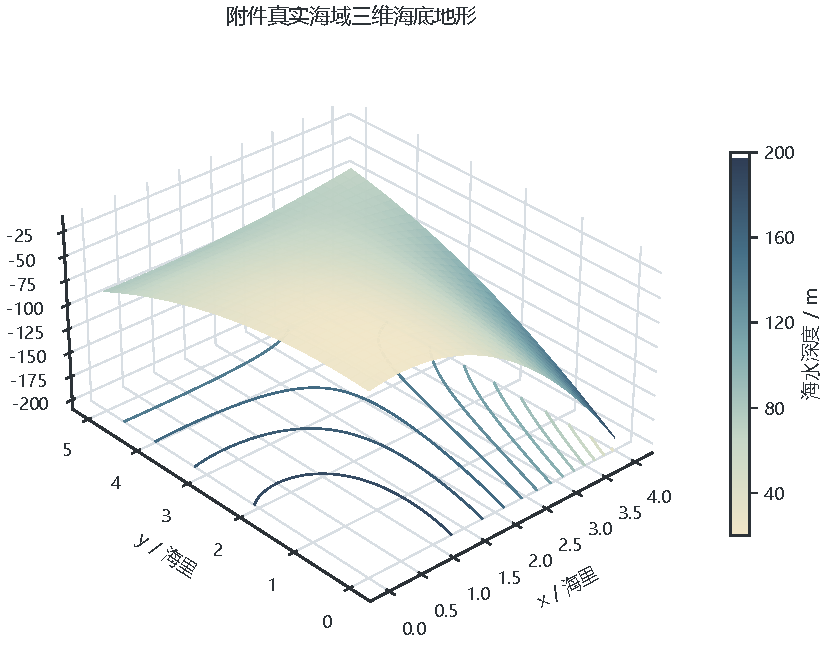
\includegraphics[width=0.8\textwidth]{../figures/q4/fig_q4_bathymetry_surface.pdf}
  \caption{真实海底总体西深东浅，南北向局部起伏要求测线按区域适应地形}
  \label{fig:q4_bathymetry_surface}
\end{figure}

\subsection{局部坡度与覆盖模型}

南北向测线的扫描剖面沿东西方向展开，左右覆盖边界主要由东西向梯度 $g_x=\partial D/\partial x$ 决定。在网格点 $(x,y)$ 邻域内，将海底近似为

\begin{equation}
  D(x+u,y)\approx D(x,y)+g_x(x,y)u.
\end{equation}

设换能器半开角为 $\phi$，声束边界与局部线性海底相交后，两侧水平半覆盖宽度为

\begin{equation}
  B_W(x,y)=\frac{D(x,y)}{\cot\phi+g_x(x,y)},\qquad
  B_E(x,y)=\frac{D(x,y)}{\cot\phi-g_x(x,y)}.
  \label{eq:q4_half}
\end{equation}

条带水平宽度为 $W_h=B_W+B_E$。对相邻测线 $x_i<x_{i+1}$，同一纵向位置 $y$ 上的局部重叠率为

\begin{equation}
  \eta_i(y)=\frac{B_E(x_i,y)+B_W(x_{i+1},y)-(x_{i+1}-x_i)}{W_h(x_{i+1},y)}\times100\%.
\end{equation}

网格点 $(x,y)$ 被第 $i$ 条测线覆盖，当且仅当
$x_i-B_W(x_i,y)\le x\le x_i+B_E(x_i,y)$。南北向梯度通过同一线段不同 $y$ 位置的水深与 $g_x$ 间接进入逐行计算。局部线性化只在网格邻域和短距离声束作用范围内有效，坡度突变区的误差由原网格回代进一步检查。

这里不用完整梯度模长替代 $g_x$。完整梯度同时包含沿航向的南北分量，而覆盖边界位于垂直航向的东西剖面；直接使用模长会把沿程水深变化重复计入横向坡度。南北起伏仍通过逐行变化的 $D(x,y)$ 和 $g_x(x,y)$ 进入每个覆盖截面。

\subsection{分条递推与候选方案生成}

将海域沿南北方向划分为水平条带。每个条带内，首条线取能够覆盖所有采样行西边界的最东位置；随后按问题三的最大允许间距向东递推，并以带内最不利位置保证相邻条带无间隙，直至覆盖东边界。不同条带独立生成测线段，合并后形成全域方案。图~\ref{fig:q4_contour} 展示 $0.50$ 海里方案的等深线、条带边界和测线位置。

“最不利位置”指使西边界覆盖或相邻条带衔接最紧的采样行，而非带内平均水深位置。以该位置递推会在其他行产生一定冗余，但可避免平均值掩盖局部浅水缺口。各条带分别求首线和后续线坐标，算法结构与问题三一致，仅将单一覆盖宽度替换为带内逐行覆盖边界。

\begin{figure}[H]
  \centering
  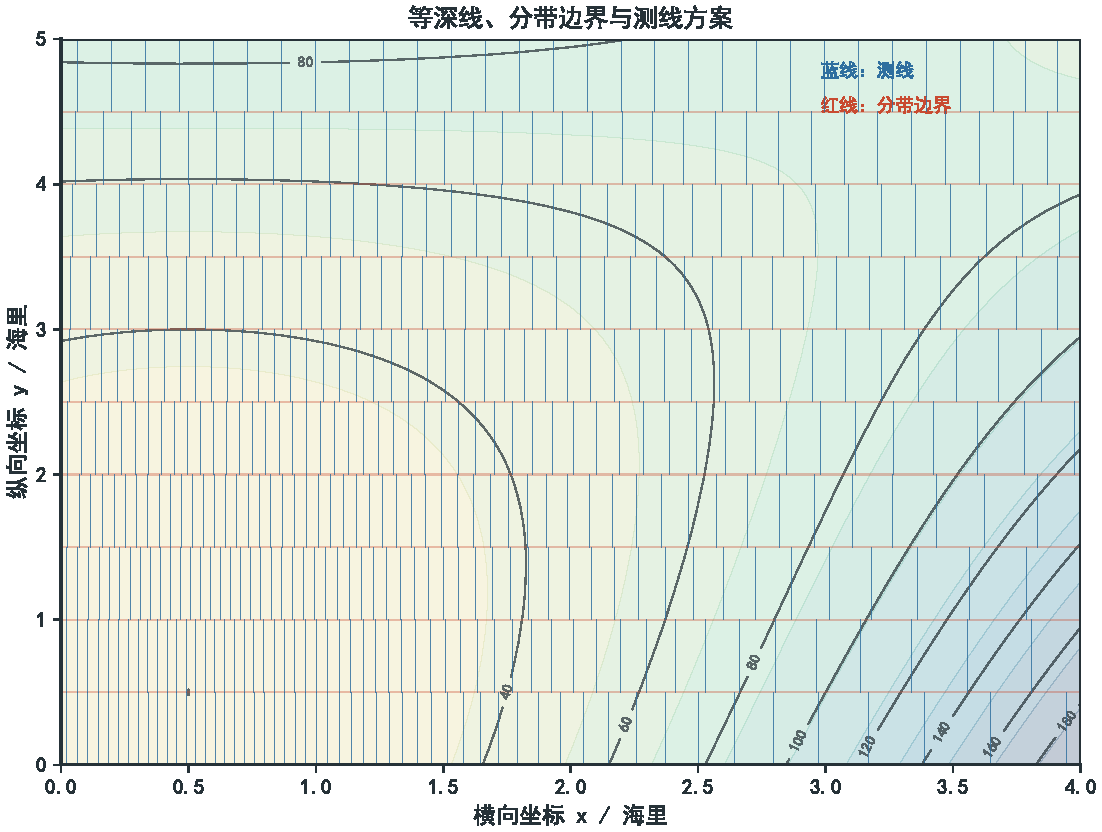
\includegraphics[width=0.8\textwidth]{../figures/q4/fig_q4_contour_route_overlay.pdf}
  \caption{$0.50$ 海里分条方案根据局部等深线调整测线位置，并覆盖东西边界}
  \label{fig:q4_contour}
\end{figure}

取 $5.00$、$1.00$、$0.50$ 和 $0.25$ 海里四种条带高度生成候选方案。四组计算保持换能器开角、测线方向、覆盖公式和网格评价方法不变；条带越短，带内最不利条件越接近局部地形，但线段数量和转场组织复杂度随之增加。

$5.00$ 海里方案把全域视为一个条带，提供不分条时的基准；其余三种尺度逐步细化南北方向的条带。候选集用于观察局部适应能力与线段组织成本的变化，不预先给任何方案附加综合权重。

\subsection{原始网格回代及指标计算}

全部候选测线生成后，返回原始 $201\times251$ 网格逐点计算覆盖和重叠。评价指标在比较结果前统一定义：总测线长度为全部实际测量线段长度之和，不含转场、调头和连接航程；漏测率为未被任何条带覆盖的原始网格点比例；平均重叠率和最大重叠率由原网格各相邻条带的 $\eta_i(y)$ 统计；超 $20\%$ 重叠长度为满足 $\eta_i(y)>20\%$ 的区段累计长度。边界覆盖、带内相邻关系和全网格复算构成三层检查。

三层检查的对象不同：边界检查确认各带首末覆盖范围封闭，带内检查确认相邻测线之间没有水平间隙，全网格检查统计离散地形上的漏测与局部重叠。若某层失败，可分别定位为边界放置、递推间距或局部线性近似问题，而不以单一汇总指标掩盖原因。

\subsection{候选方案比较与最终选择}

四种分条尺度的回代结果见表~\ref{tab:q4}。

\begin{table}[H]
  \centering
  \caption{不同分条尺度下的覆盖、冗余与线段组织成本}
  \label{tab:q4}
  \resizebox{\textwidth}{!}{%
    \begin{tabular}{lccccc}
      \toprule
      方案 & 线段数 & 总长度 / m & 漏测率 / \% & 超 $20\%$ 重叠长度 / m & 最大重叠率 / \% \\
      \midrule
      全域 $5.00$ NM & 60  & 555600.00 & 0.00 & 276877.69 & 76.42 \\
      $1.00$ NM      & 240 & 444480.00 & 0.00 & 51525.55  & 45.86 \\
      $0.50$ NM      & 461 & 426886.00 & 0.00 & 5481.92   & 49.01 \\
      $0.25$ NM      & 897 & 415311.00 & 0.00 & 2742.38   & 46.07 \\
      \bottomrule
    \end{tabular}%
  }
\end{table}

四种方案的漏测率均为 $0.00\%$。分条从 $5.00$ 海里细化到 $0.25$ 海里时，总长度由 $555.600$ km 降至 $415.311$ km，超 $20\%$ 重叠长度由 $276877.69$ m 降至 $2742.38$ m，线段数则由 60 增至 897。细分减弱了全带最不利水深的限制，同时提高了作业组织成本。

按题面直接要求的总长度、漏测率和超重叠长度，$0.25$ 海里方案是四个候选方案中的数学指标最优方案。若考虑题面未计入的转场与调头负担，$0.50$ 海里方案将线段数由 897 降至 461，总长为 $426.886$ km，超重叠长度为 $5481.92$ m，平均相邻重叠率为 $4.66\%$，可作为工程折中。该推荐不等同于单项数学指标的唯一最优解。

从 $0.50$ 海里进一步细化至 $0.25$ 海里，总长度由 $426.886$ km 降至 $415.311$ km，超重叠长度由 $5481.92$ m 降至 $2742.38$ m，但线段数由 461 增至 897。题面未给出船速、转弯半径或单次调头耗时，无法把组织成本折算为统一费用；因此表格保留原始指标，工程推荐只作为有条件的折中判断。

\subsection{局部重叠超限及适用边界}

$0.50$ 海里方案回代后的覆盖率为 $100\%$，但最大局部重叠率为 $49.01\%$，超限主要集中在局部坡度变化较大及各条带独立递推的边界附近。平均重叠率较低，源于多数区段按覆盖完整性控制间距，而少量极端位置贡献了较高最大值；因此平均值、累计超限长度和局部最大值需同时报告。

分条边界两侧的测线由相邻条带分别递推，地形条件和首线位置可能不同，因而容易出现局部覆盖叠加；坡度突变又会使左右半宽在短距离内快速变化。两类因素增加局部最大值，但原网格回代显示其未造成覆盖缺口。超限累计长度用于衡量这部分冗余的空间规模。

当前方案保证原始网格点无漏测，并以累计长度衡量局部冗余，未要求每一点均满足 $10\%\sim20\%$。若将 $20\%$ 设为逐点硬约束，需要重新调整条带边界或局部测线位置；坡度突变、网格间细尺度地形及声速分层也会降低局部线性模型的精度。上述因素限定了方案作为测前规划的适用范围。

原网格漏测率 $0.00\%$ 只说明给定采样点均被覆盖，不能排除采样间隔内存在未解析的细小地形突变。实际作业应结合实时水深、姿态和声速信息复核覆盖边界，并在高坡度区和分条接缝附近预留更高安全重叠率。
